\chapter{Supervised Progressive Autonomous Robot \newline Competencies}\label{chap:sparc}
\glsresetall
\graphicspath{{images/sparc/}}

\begin{framed}
	\textbf{Key points:}
	%CHeck for 
	\begin{itemize}
		\item Novel interaction framework to teach robots an action policy while interacting.
		\item A human teacher is in control of the robot's actions whilst the robot learns from this supervision.
		\item The robot proposes actions to be executed to the teacher.
		\item The teacher provides feedback on intentions rather than actions.
		\item The robot's behaviour (under supervision) can be assumed to be optimal.
		\item Workload on the teacher decreases over time as the robot learns.
	\end{itemize}
\end{framed}

Parts of the work presented in this chapter have been published in \cite{senft2015sparc} and \cite{senft2017supervised}. The final publications are available from Springer and Elsevier:
\begin{itemize}
	\item \url{http://dx.doi.org/10.1007/978-3-319-25554-5_60}.
	\item \url{https://doi.org/10.1016/j.patrec.2017.03.015}.
\end{itemize}

\newpage

As presented in Chapter \ref{chap:background}, robots would profit from being able to learn from human teachers how to interact with other humans. Using \gls{iml} to achieve this transfer of social and task knowledge from the human domain-expert to the robot would result in a faster and safer learning than slow iterative update of behaviours by engineering the action policy, learning from large quantities of data or by trials and errors as with \gls{rl}.

However, as stated in this previous chapter, \gls{iml} is seldom applied to learning to interact with humans. No current system provides the teacher with enough control over the robot's actions to validate the first principle (Section \ref{ssec:back_constraints}: `Only execute appropriate actions'). Techniques relying solely on feedback from the teacher cannot prevent the robot to execute an incorrect action, but only reduce the chances of future errors by rewarding negatively incorrect actions after their execution \citep{senft2017supervised}. Similarly, with current techniques based on \gls{lfd} the teacher relinquishes its control over the robot when not demonstrating, only reacting in hindsight after the learner makes mistakes and its erroneous actions have impacted the real world \citep{chernova2009interactive}.

In order to provide a robot with an appropriate action policy, adaptive to different context or behaviours and requiring a low workload on the teacher or supervisor, in \cite{senft2015sparc} we introduced the \gls{sparc} framework of interaction. \gls{sparc} allows end-users to safely teach a robot an action policy applicable to \gls{hri}.
\section{Frame}

Similarly to other applications of \gls{iml}, SPARC requires inputs from a teacher to learn an action policy to interact with the world. In this framework, the robot interacts with two entities: the target and the teacher, which results into two intertwined interactions: the application interaction (task the robot learns to achieve) and the teaching interaction (relation with the teacher), as shown in Figure \ref{fig:frame}. In the generic case, the overall interaction is a triadic interaction (Teacher - Robot - Human target or Teacher - Robot - Environment), such as teaching a robot tutor to support child learning (as implemented in Chapter \ref{chap:tutoring}). But in specific cases, the overall interaction can be only dyadic (Teacher - Robot), such as a robot at home learning from its user how to support them better.

\begin{figure}[ht]
	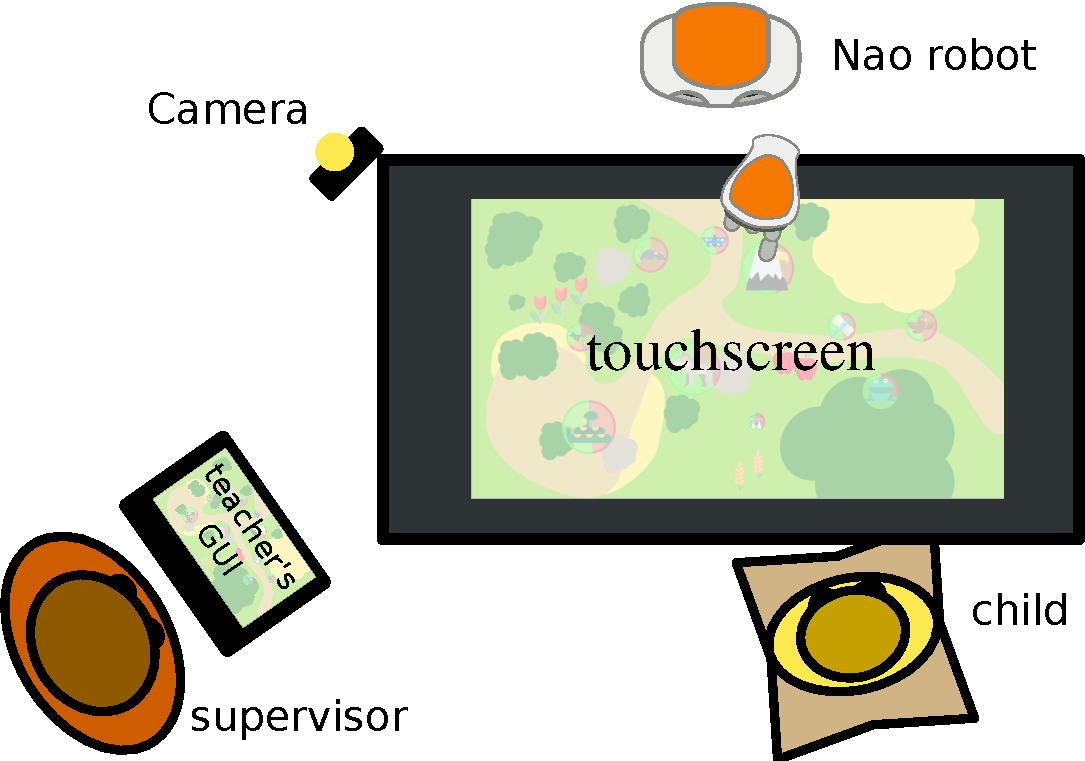
\includegraphics[width=.8\linewidth]{setup.pdf}
	\centering
	\caption{Frame of the interaction: a robot interacts with a target, suggests actions and receive commands and feedback from a teacher. The robot uses machine learning to improve its suggestions over time.}
	\label{fig:frame}
\end{figure}

\section{Principles} \label{sec:sparc_principles}

\gls{sparc} defines an interaction between a learner (virtual agent or robot) and a teacher following these principles:
\begin{itemize}
	\item The learner has access to a representation of the state of the world and a set of actions.
	\item The teacher can select actions for the robot to execute.
	\item The learner can propose actions to the teacher before executing them (informing them about its intentions) .
	\item The teacher can enforce or cancel actions proposed by the learner and actions non evaluated are implicitly validated and executed after a short delay.
	\item The learner uses \gls{ml} to improve its action policy using the teacher's commands and feedback on propositions.
\end{itemize} 

This interaction between the learner and the teacher is similar to the level 6 on the Sheridan scale of autonomy: "computer selects action, informs human in plenty of time to stop it" \citep{sheridan1978human} with the addition that the human has the opportunity to select actions for the agent to execute. In this thesis, we will refer to this interaction as `\gls{sa}': the robot interacts autonomously under the supervision of a human who can ensure that the behaviour is constantly appropriate.

This way of keeping a human in the learning loop and with the opportunity to override the agent actions and the robot learning from these demonstrations is similar to Dogged Learning \citep{grollman2007dogged}. However, with \gls{sparc}, this ability to provide demonstrations is combined with \gls{sa}. This results in a mixed control system where the teacher can select actions and have the robot perform them while the robot only proposes actions to the teacher. In response to this suggestion, the teacher has the choice between pre-empting the action or let it be executed. A learning algorithm on the robot side uses the feedback and commands from the teacher to improve the correctness of the suggested actions until reaching an efficient action policy. This learning mechanism coupled with auto-execution of actions aims to decrease over time the requirement of interventions from the teacher, thus reducing the workload on the teacher as the robot learns. The diagram presented in Figure \ref{fig:sparc_diagram} and the flowchart in Figure \ref{fig:sparc_flowchart} present in a graphical way this interaction between the learner and the teacher.

\begin{figure}[ht]
	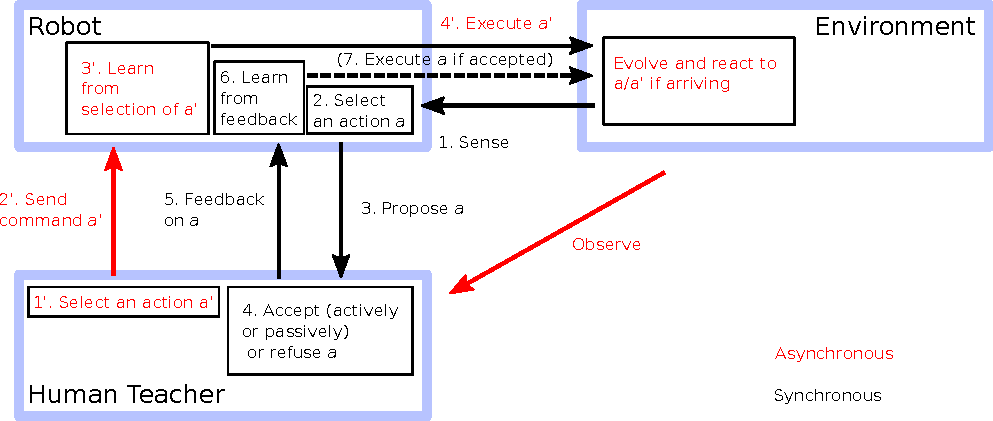
\includegraphics[width=1\linewidth]{diagram.pdf}
	\centering
	\caption{Diagram of interaction between the robot, the human teacher and the environment with \gls{sparc}: synchronously, the robot can propose actions to the teacher that evaluated (approved or cancelled) and the teacher can select actions to be executed in an asynchronous fashion.}
	\label{fig:sparc_diagram}
\end{figure}

Additionally, keeping the human in the loop also gives them the opportunity to provide additional information to the algorithm speeding up the learning. The main difference between \gls{sparc} and Dogged Learning or CBA \citep{chernova2009interactive} is the communication of intentions and full control of the teacher over the robot's action with \gls{sparc}. The teacher is informed beforehand of the robot future actions and can prevent them before the execution, which provides more control on the robot's action policy compared to other \gls{iml} methods. The teacher does not have to correct an action after it has impacted the world, but can pre-empt incorrect actions using the intention or suggestion transmitted by the robot. The agent learns to avoid actions with expected negative impact without having to face the results of the execution of these undesired actions. This implies that the behaviour executed by the robot can be assumed to be optimal, potentially simplifying the learning mechanism.

\begin{figure}[ht]
	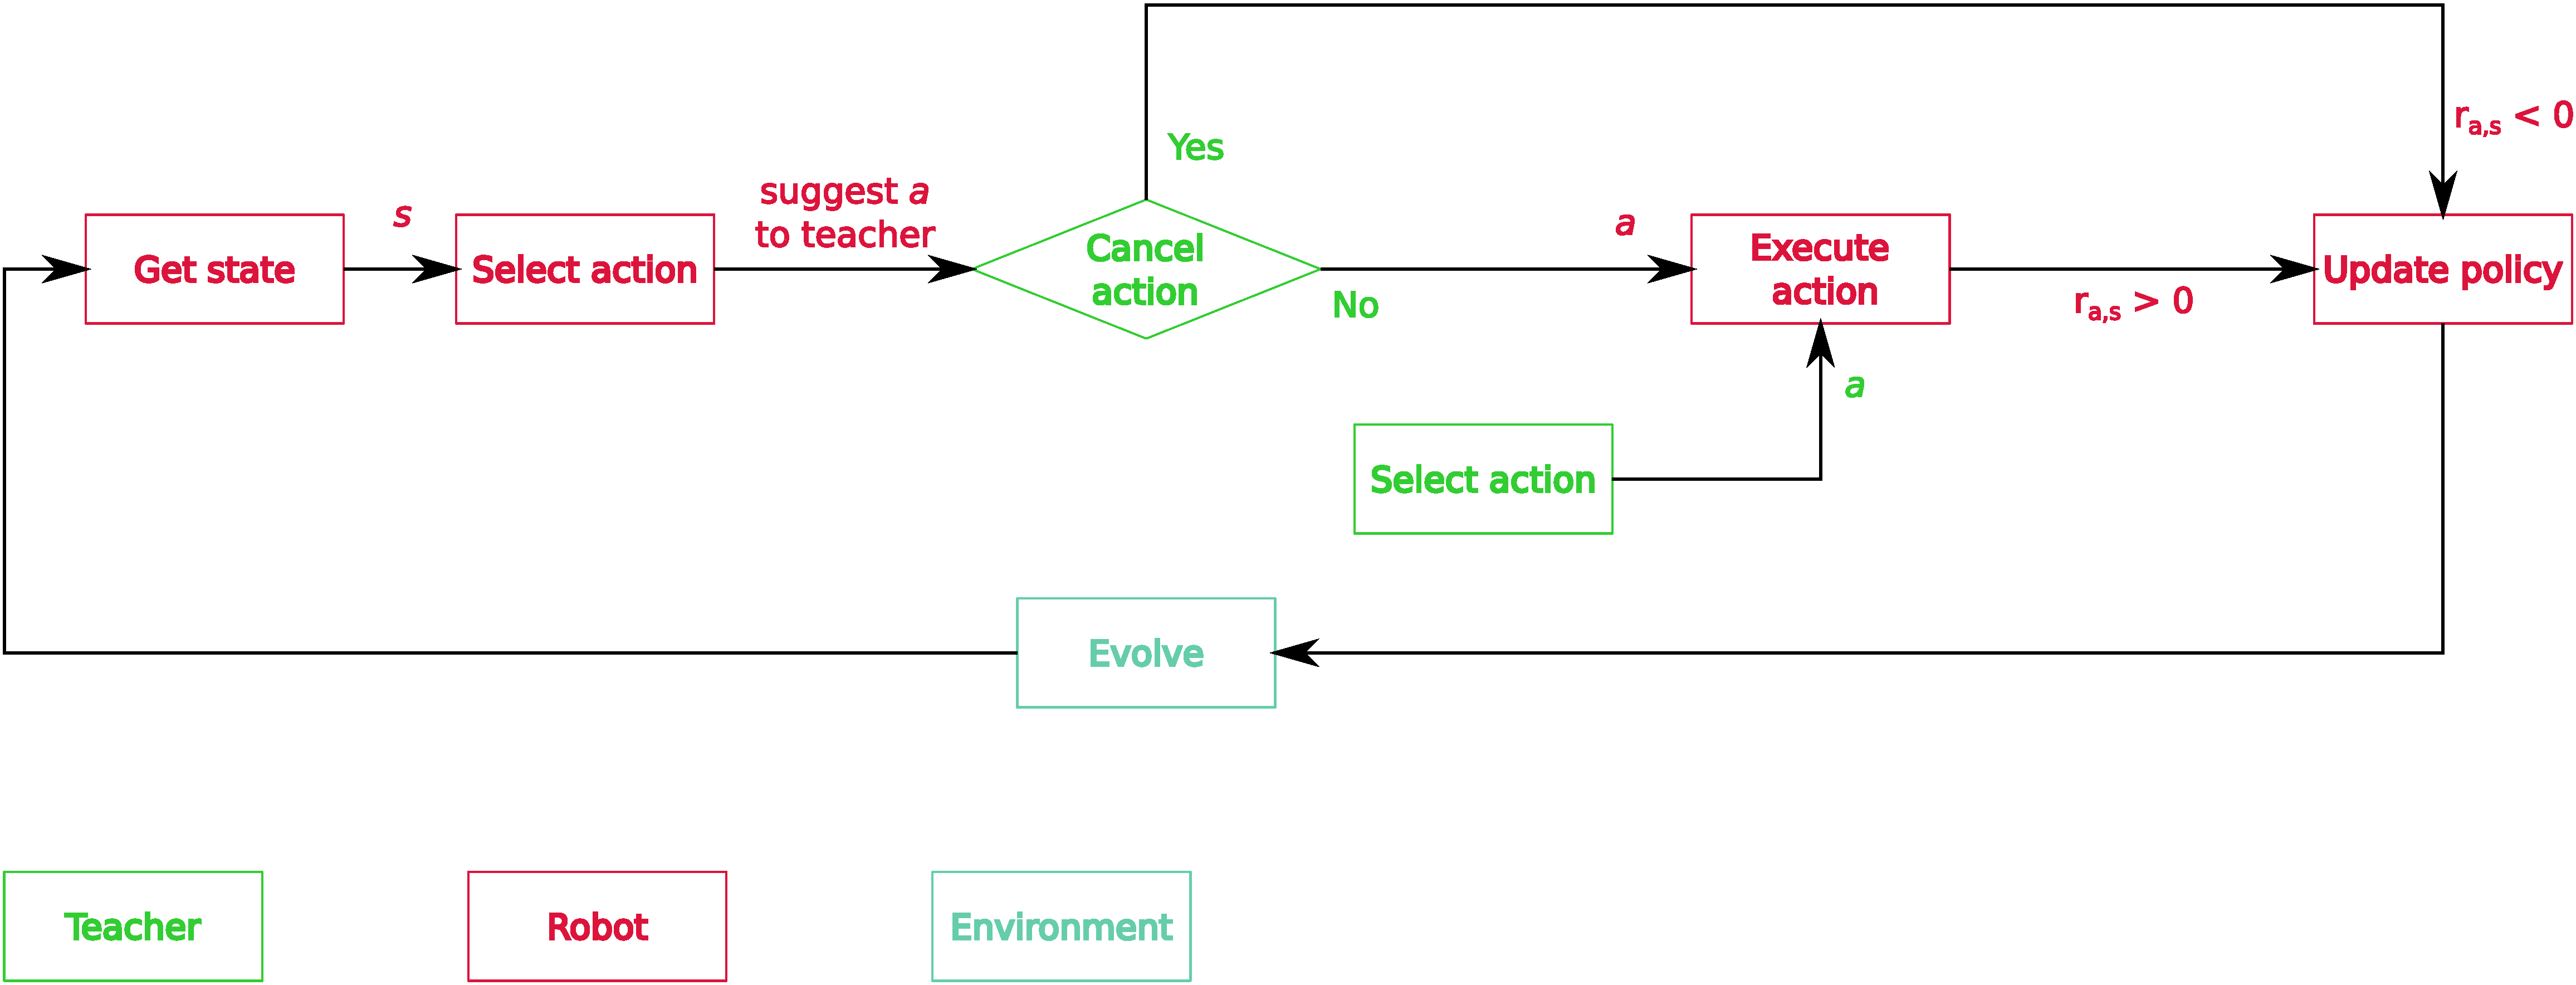
\includegraphics[width=1\linewidth]{flowchart.pdf}
	\centering
	\caption{Flowchart of the action selection loop between the robot and the teacher.}
	\label{fig:sparc_flowchart}
\end{figure}

This approach is comparable to predictive texting as seen on phone nowadays. The user can select the words proposed by the algorithms (or implicitly accept them by pressing space) or write their own. The algorithm learns the user's preferences and habits and aims to suggest words more and more appropriate to the user. However, predictive texting aims mostly to correct users' errors and interact in static environments. And \gls{sparc} aims to replicate a teacher's action policy in continuous time, in a dynamic interactive environment evolving both dependently and independently of the agent actions.

Alternatively, \gls{sparc} can be seen as a way to provide pro-activity to the robot. By observing interactions on a larger time scale, such as an assistant robot at home, \gls{sparc} allows the agent to propose help when the current state is similar to previous observation. This would be to compare to an operated robot where each action executed by the robot would have to be requested by the user. By proposing actions to the teacher, the robot takes the initiative to support humans, while not imposing its presence in the environment: executing actions without informing the surrounding humans could be perceived as rude or annoying.

\section{Goal}

\gls{sparc} aims to provide an interaction framework to teach robots an action policy possessing the following characteristics:
\begin{itemize}
	\item Usable by people without expertise in computer science.
	\item Fast policy learning from in-situ guidance.
	\item No constant requirement of human input to act in the world.
	\item Robot's behaviour constantly appropriate.
\end{itemize}

Figure \ref{fig:concept} presents an idealistic comparison of the expected workload, performance and autonomy of four methods: autonomous learning (e.g. \gls{rl} - \citealt{sutton1998reinforcement}), feedback based teaching (e.g. TAMER - \citealt{knox2009interactively}), \gls{woz} and \gls{sparc}. Unlike other methods, by following the principles presented in Section \ref{sec:sparc_principles}, \gls{sparc} is expected to maintain a constant high performance even during early stages of learning. In later stages of the learning, the workload on the human teacher should decrease as the agent improves its action policy, making its suggestions more accurate.

\begin{figure}[ht]
	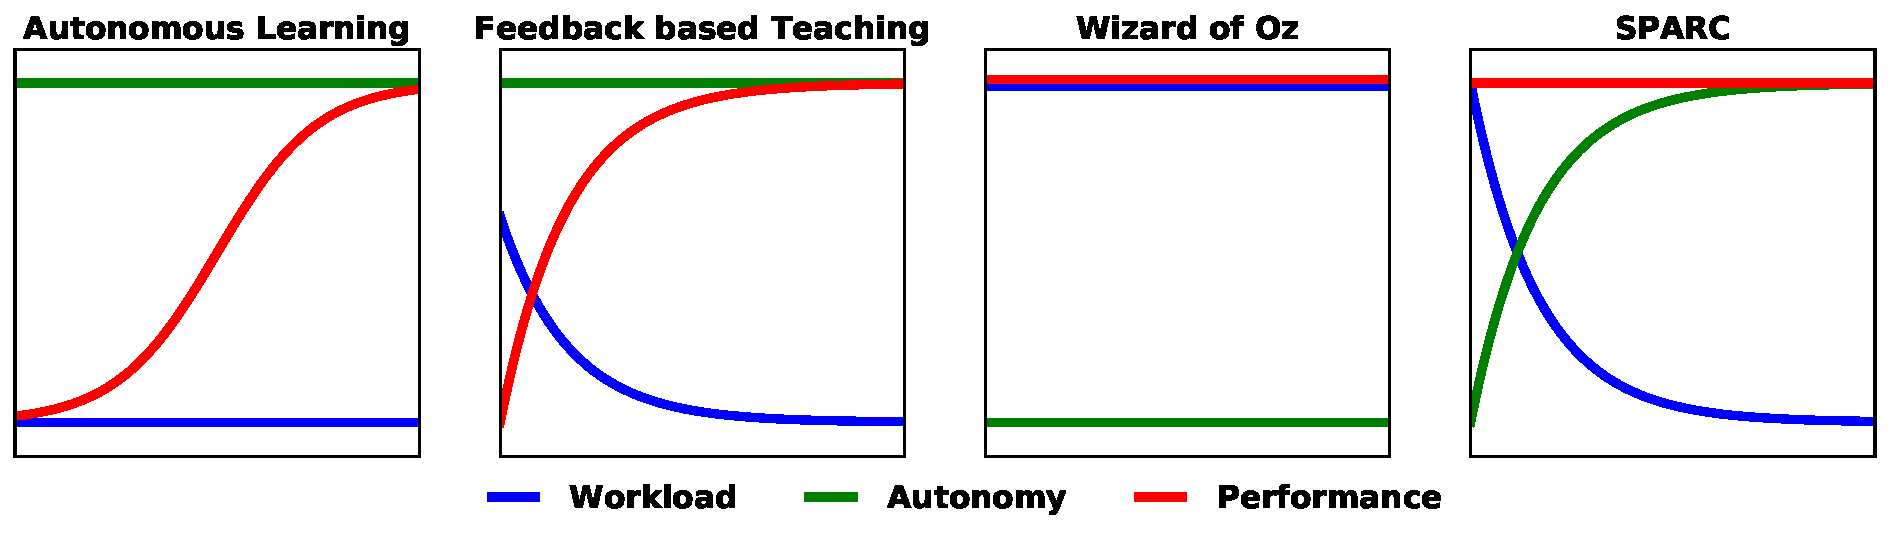
\includegraphics[width=1\linewidth]{concept.pdf}
	\centering
	\caption{Idealistic evolution of workload, performance, and autonomy over time for autonomous learning, feedback-based teaching, \gls{woz} and \gls{sparc}.}
	\label{fig:concept}
\end{figure}

Once the behaviour is deemed appropriate enough by the teacher, the agent is ready to be deployed to interact autonomously in the real world if this outcome is desired. Alternatively, in contexts where a human expert still cannot be removed from the control loop, such as \gls{rat}, a supervisor stays in control of the robot's actions in a \gls{sa} fashion. Similarly to the teaching phase, the robot informs the supervisor of its actions and the human only has to intervene in case of incorrect propositions. While still requiring attention from the supervisor, this reduction of human actions to control the robots aims at reducing the workload on the supervisor. As the supervisor has a better knowledge of the agent's behaviour, they can be especially careful in cases when they know the agent is prone to making errors. And as the control of the agent requires less effort from the supervisor, they can focus more closely on the application interaction than the teaching one in the other cases. 
%This approach is similar to safety drivers behind autonomous vehicles but with information about the car's intentions rather than solely observing the car's actions. 
%MAybe something on knowing critical parts of the interaction policy (Example DREAM only evaluation of performance)

\section{Implications}

Similarly to other \gls{iml} approaches, the requirement of a human in the action selection loop limits the time scale of interaction and this effect is an important consideration when applying \gls{sparc} to an interaction. With this type of \gls{iml}, three time scales are coexisting: the robot's, the teacher's and the interaction's. The robot has an internal clock running probably multiple times per second, sensing the world and deciding if an action should be provided. The human teacher has to be able to cancel actions before their executions, so they needs to be provided with few seconds to react to propositions, which reduces the rate of actions selection to 0.5 Hz or below. Depending of the application, actions might have to be executed in a time critical environment (such as driving) or less critical ones (such as an assistant robot at home supporting a person). This means that the width of actions' acceptance window impacts the usability of \gls{sparc}. To be applicable, an acceptance window needs to span few seconds to have the actions being valid both when proposed by the robot and when accepted by the teacher. The difference of time scales and the requirement of time allocated for the teacher to react reduce the application of \gls{sparc} compared to other \gls{iml} methods. However, this limitation of application is the price to pay to ensure the appropriateness of actions, and this effect can be mitigated by using higher level actions or applications less critical in term of time.  % and this has the advantage to ensure that only correct actions will be executed without requiring the human to select them all.

\gls{sparc} is an \gls{ilfd} method (cf Section \ref{ssec:back_ilfd}) and as such presents many similarities with other non-interactive \gls{lfd} (cf. Section \ref{ssec:back_lfd}) as it uses human demonstrations of policies to learn. However, most of the applications of \gls{lfd} \citep{argall2009survey,billard2008robot} are focused on learning a manipulation skill in a mostly deterministic environment. \gls{lfd} has seldom been used to teach an action policy to interact with humans \citep{liu2014train,sequeira2016discovering,munzer2017efficient} and never in an online fashion. Munzer et al. proposed an interactive planner that would learn offline the current user's preferences and desires, but two key differences exist between this approach and \gls{sparc}. The learning planner is well suited to clearly defined environments (e.g. \gls{hrc}) where a similar task with clear steps has to be done multiple times. As such the learning can happen offline between the repetitions. \gls{sparc} is defined to be applicable to non-linear environments where learning should happen online in tasks without clear start and ending states. Secondly, using a threshold, Munzer et al. define actions with low risk which are executed (and can be cancelled during the execution) and actions with higher risk which have to be validated first by the human. \gls{sparc} does not make this distinction, but proposes both types of actions to the teacher and will start executing them if no feedback is received. This removes the  need for the human to explicitly approve a correct action if proposed while ensuring that the human can cancel incorrect action before their execution. This principle aims to reduce the number of required interventions from the human to teach the robot compared to methods as the one presented by Munzer et al. 

Additionally, \gls{sparc} differs from Active Leaning (cf. Section \ref{ssec:back_active}) by the fact that the agent cannot decide which sample will be evaluated by the teacher. As the robot interacts with humans, the datapoints provided to the teacher for \textit{labelling} emerge from the interaction, and cannot be selected at will. 
    
%\section{Implications}

%The principles described in section \ref{sec:sparc_principles} have also implications on the interactions between the teacher and the agent and between the agent and the environment. As the teacher has the power evaluate the actions proposed by the agent before their execution, it actually evaluates the intentions of the agent rather than its behaviour. This difference is key as traditional \gls{iml} approaches only evaluate the actions a posteriori by their effects. This implication is fundamental in \gls{hri} as a robot executing non appropriate actions when interacting with humans should not be deployed (cf. first principle in Section \ref{ssec:back_constraints}) and asing the evaluation of the teacher on the intention rather than waiting for the action's outcome gives the opportunity to the teacher to pre-empt incorrect actions preventing the execution of undesired behaviours. The agent learns to avoid actions with expected negative impact without having to face the results of the execution of these undesired actions.

%Most importantly, the control given to the teacher on the agent's actions ensures that every action executed by the learner in the world has been either actively or passively validated by the teacher. This implies that each action executed can be assumed to be appropriate to the current state, potentially simplifying the learning algorithm.

\section{Interaction with Machine Learning Algorithms}

The principles of \gls{sparc} define it at the crossroads between \gls{sl} and \gls{rl}. \gls{sparc} can be used in two ways: either to reproduce a teacher's policy in a supervised fashion or to discover a useful action policy using the teacher to bias the exploration, limiting errors and only interacting in desired parts of the environment.

As such, \gls{sparc} only defines an interaction framework between a teacher and a learner, and is agnostic to the learning mechanism: it can be combined with any algorithms used in \gls{sl} or \gls{rl}. This research explored combinations with three types of algorithms: supervised learning using a feed-forward neural network (Chapter \ref{chap:woz}), reinforcement learning (Chapter \ref{chap:control}), and supervised learning using an instance based algorithm (Chapter \ref{chap:tutoring}). However \gls{sparc} could be combined with a wide range of other algorithms.


Similarly to Inverse Reinforcement Learning \citep{abbeel2004apprenticeship} or other techniques combining \gls{rl} and \gls{lfd} \citep{billard2008robot}, if used with a reward function \gls{sparc} could go beyond the demonstrated action policy and achieve a performance higher than the demonstration. However this aspect has not been evaluated in this work.

\section{Summary}
    
This chapter introduced \acrfull{sparc}, a novel interaction framework to teach agents an action policy. This approach is suited to teach a robot to interact with humans as it validates the principles defined in Section \ref{ssec:back_constraints}. \gls{sparc} starts in a similar fashion to \gls{woz}: the teacher selects actions at any time to be executed by the robot. Then, using a learning algorithm, the agent starts to propose actions to the teacher who can let them be executed after a short time or cancel them if not appropriate. This mechanism combining selections, suggestions, and evaluations ensures the appropriateness of actions as a human could have pre-empted any inappropriate action before their execution. This additionally provides the adaptivity as the teacher can extend the behaviour beyond the current action policy. The learning algorithm associated with the auto-executions ensures that once the robot starts to learn, the human workload decreases. When an acceptable action policy is reached, the robot is ready to be deployed to interact autonomously if this outcome is desired.
